\documentclass[11pt]{article}

\usepackage[a4paper,margin=2.2cm]{geometry}
\usepackage{graphicx}
\usepackage{booktabs}
\usepackage{amsmath}
\usepackage{amssymb}
\usepackage{caption}
\usepackage{subcaption}
\usepackage{float}
\usepackage[hidelinks]{hyperref}
\usepackage{xcolor}
\usepackage{enumitem}
\setlist{nosep,leftmargin=1.4em}
\captionsetup{font=small,labelfont=bf}
\graphicspath{{images/}}

\begin{document}

% ----------------------------------------------------------------------
% Title page
% ----------------------------------------------------------------------
\begin{titlepage}
\centering
\vspace*{\fill}


\includegraphics[width=0.38\linewidth]{images/upc-positiu-p3005.png}\\[2.4cm]

{\LARGE\bfseries Predicting Term-Deposit Subscription\\[0.3cm]
on the Bank Marketing Dataset\par}

\vspace{0.7cm}
{\large\itshape A Complete Machine-Learning Pipeline\par}

\medskip

{\large\itshape Data Science — ML Project 2026\par}

\vspace{0.9cm}
\rule{0.35\linewidth}{0.4pt}

\vspace{0.9cm}
{\large Arman Bazarchi\par}

\vspace*{\fill}
\end{titlepage}

% ----------------------------------------------------------------------
% Table of contents
% ----------------------------------------------------------------------
\newpage
\tableofcontents
\thispagestyle{empty}
\newpage
\setcounter{page}{1}

\section{Introduction and Problem Description}
A Portuguese bank ran a tele-marketing campaign and for each contact recorded client attributes,
campaign details, and the macro-economic situation at the time of the call. The task is binary
classification: will the client subscribe to a term deposit (\texttt{y}~$\in\{$no,yes$\}$)? The dataset
satisfies the project requirements --- it is real, has 20 features (10 numerical, 10 categorical) and
41{,}188 samples, and needs non-trivial preprocessing.

\medskip

 

Two properties make this an interesting dataset rather than trivial. First, it is \textbf{heavily imbalanced}
(88.7\% ``no'' / 11.3\% ``yes'', a $\approx 7.9{:}1$ ratio), so accuracy is not reliable and the minority
class is what we are interested in. Second, the dataset shows that \texttt{duration} (call length) is
\textbf{target leakage}: it is only known \emph{after} the call ends, so although it is the single
strongest correlate of the target, it cannot be used by a realistic predictor. Our objective is not to maximise a score but to analyze, justify, and interpret every step to find interesting insights about which signals actually drive subscription.


\begin{table}[H]
\centering\small
\caption{Key features list.}
\label{tab:features}
\begin{tabular}{l l p{7cm}}
\toprule
Feature & Type & Overview / interpretation \\
\midrule
\texttt{y (Target)} & binary & whether the client subscribes to a term deposit (yes/no). \\
\midrule
\multicolumn{3}{l}{\emph{Macro-economic block, collinear ($|r|>0.9$)}}\\\\
\texttt{euribor3m}      & numeric & 3-month Euribor interbank rate, proxy for how attractive market alternatives are. \\
\texttt{emp.var.rate}   & numeric & Quarterly employment variation rate. \\
\texttt{nr.employed}    & numeric & Number of employees economy-wide. \\
\texttt{cons.price.idx} & numeric & Consumer price index. \\
\texttt{cons.conf.idx}  & numeric & Consumer confidence index, mostly absorbed by the block. \\
\midrule
\multicolumn{3}{l}{\emph{Campaign history --- the second driver}}\\\\
\texttt{poutcome} & ordinal & Outcome of the previous campaign. \\
\texttt{previous} & numeric & Number of contacts before this campaign. \\
\texttt{contact}  & binary  & Contact channel, by cellular or telephone. \\
\texttt{campaign} & numeric & Contacts during this campaign. \\
\texttt{month}    & nominal & some months (e.g.\ Mar, Sep, Oct, Dec) show higher subscription rates. \\
\midrule
\multicolumn{3}{l}{\emph{Special cases and weak signal}}\\\\
\texttt{duration} & numeric & Call length, excluded as leakage. \\
\texttt{pdays}    & numeric & Days since last contact, 999 if never contacted. \\
\texttt{age}      & numeric & Client demographic. \\
\bottomrule
\end{tabular}
\end{table}



\paragraph{Pipeline overview.} All phases share one preprocessed output and a fixed 80/20 stratified
split (\texttt{random\_state=42}). Imbalance is handled \emph{inside} the models (class weights or by giving
balanced sample weights), never by resampling the test set. We report Accuracy, F1, ROC-AUC and AUPR,
because the task is classification, the regression metrics (R\textsuperscript{2}, MAE, RMSE) do not
apply (in Phase~II Ridge/Lasso we apply a didactic Linear-Probability-Model aside, not our main task).

\newpage

\section{Data and Preprocessing}
\paragraph{Exploratory analysis.} The target is strongly skewed: a naive
``always-no'' model would already score $\approx 89\%$ accuracy while being useless, which is why we lead
with F1/ROC-AUC/AUPR. The correlation matrix reveals two structural facts that
appears repeatedly throughout the project:

\medskip

\begin{itemize}
\item \textbf{Severe multicollinearity in the macro block:} features \texttt{euribor3m}, \texttt{emp.var.rate}, and \texttt{nr.employed} are correlated at $|r|>0.9$ ---  they are different readings of the same economy situation.

\medskip

\item \textbf{The usable signal is moderate:} after the leaky \texttt{duration} ($r=0.41$), and the redundant 
\texttt{pdays} ($r=-0.32$, comparably strong but dropped anyway), the strongest usable correlates are \texttt{nr.employed} ($-0.35$), \texttt{euribor3m} ($-0.31$) and \texttt{emp.var.rate}
($-0.30$), all negative (a strong economy decreases chance of subscription), then \texttt{previous}
($+0.23$). Client demographics such as \texttt{age} ($r=0.03$) are nearly uncorrelated with the target.
\end{itemize}


\begin{figure}[H]
\centering
\begin{subfigure}{0.31\linewidth}
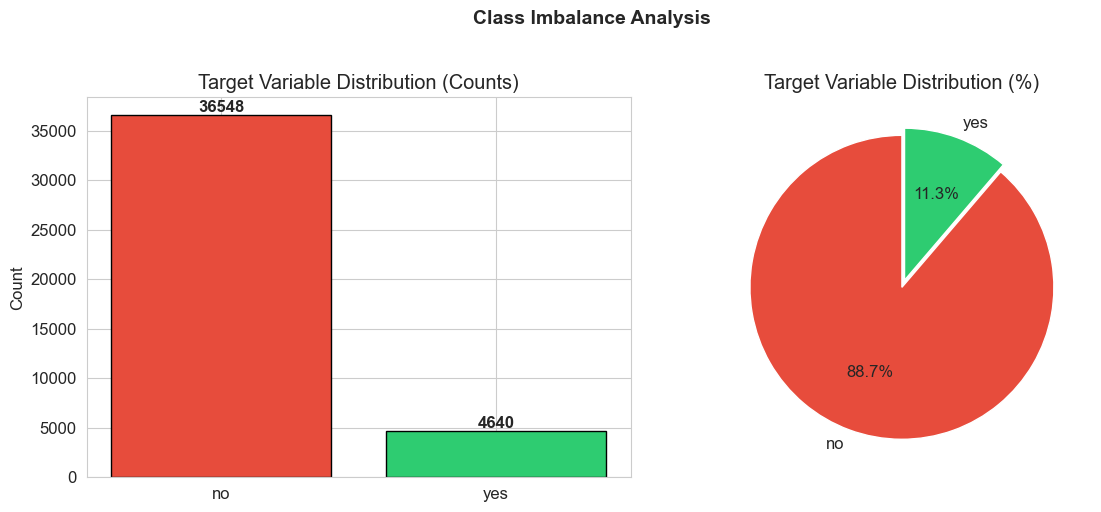
\includegraphics[width=\linewidth]{preprocessing_1.png}
\caption{Class imbalance (11.3\% yes).}\label{fig:imbalance}
\end{subfigure}\hfill
\begin{subfigure}{0.66\linewidth}
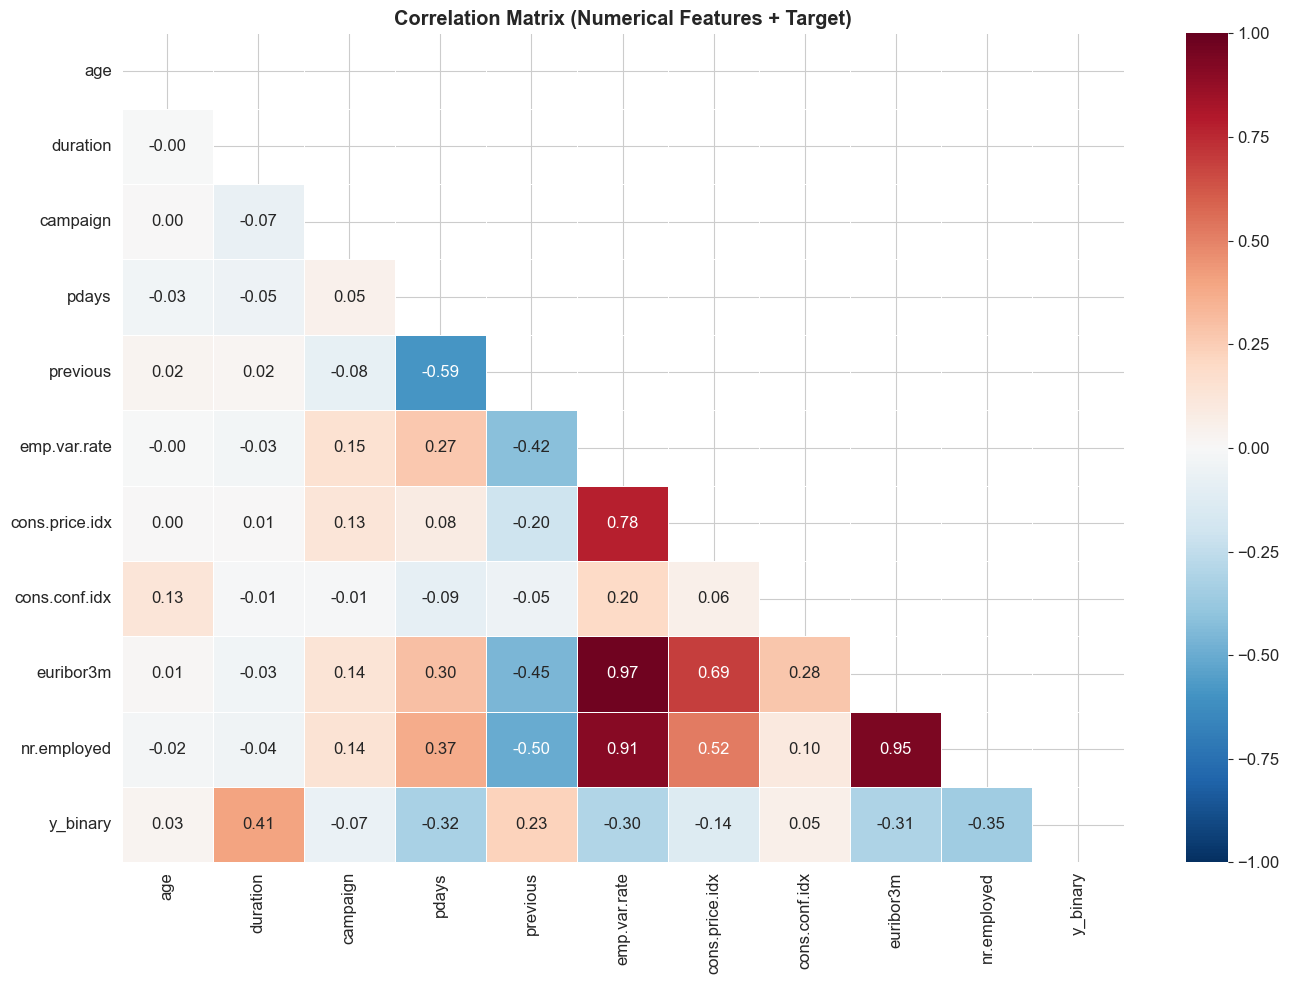
\includegraphics[width=\linewidth]{preprocessing_4.png}
\caption{Correlation matrix: the macro block is correlated ($|r|>0.9$), usable target
correlations are weak and negative.}\label{fig:corr}
\end{subfigure}
\caption{Exploratory data analysis.}
\end{figure}


\paragraph{Preprocessing decisions.} For categorical features, we treat \texttt{"unknown"} as its own category (it may carry
information, like clients who refuse to provide credit-default status), since dropping the 20.9\% of
rows with unknown \texttt{default} would be wasteful. We apply type-aware encoding rather than simple
one-hot: \emph{ordinal} for \texttt{education} and \texttt{poutcome} (since they have a natural order),
\emph{binary} for \texttt{contact}, \emph{integer} (0/1/2) for the binary + "unknown" features, and
\emph{one-hot} (in the modelling notebooks) for the genuinely nominal \texttt{job}, \texttt{marital},
\texttt{month}, \texttt{day\_of\_week}. Numeric features are standardized, tree models are scale-invariant but we
keep one consistent matrix for all phases.

\paragraph{Dropping \texttt{pdays}.} Since 96.3\% of \texttt{pdays}(number of days passed since last contact) values are the sentinel $999$
(meaning ``never contacted''). However, `pdays=999` also appears in records where `previous(number of times client was contacted before)` \textgreater 0 and also `poutcome(outcome of the last call)` indicates a real outcome (failure/success and not nonexistent), suggesting the 999 might also be used as "not available" rather than strictly "never contacted"(but we are not sure about it), and only 3.7\% (1{,}515 rows) are real day-counts. Imputing the 4{,}110 ``contacted but untracked'' rows from just 1{,}515 samples would invent more data than it recovers, and the
campaign-history signal is already captured by \texttt{poutcome} (outcome) and \texttt{previous}
(contact count). We therefore \textbf{drop} \texttt{pdays}, a well-justified removal beats a fragile imputation.

\paragraph{Outliers.} An IQR analysis flags extremes in \texttt{previous}
(13.7\%), \texttt{duration} (7.2\%), \texttt{campaign} (5.8\%) and \texttt{age} (1.1\%), while the macro
indicators have \emph{zero} outliers. Importantly these seem \textbf{true values, not data-entry errors} (the \texttt{previous}/\texttt{pdays} flags come from many zero or sentinel values, \texttt{campaign} up to 56 contacts, and \texttt{age} up to 98 are real). We therefore \textbf{keep all rows}: deleting them would discard real signal, also mostly our models are outlier-invariant, and the linear/kernel models are already standardized and regularized.



\begin{figure}[H]
\centering
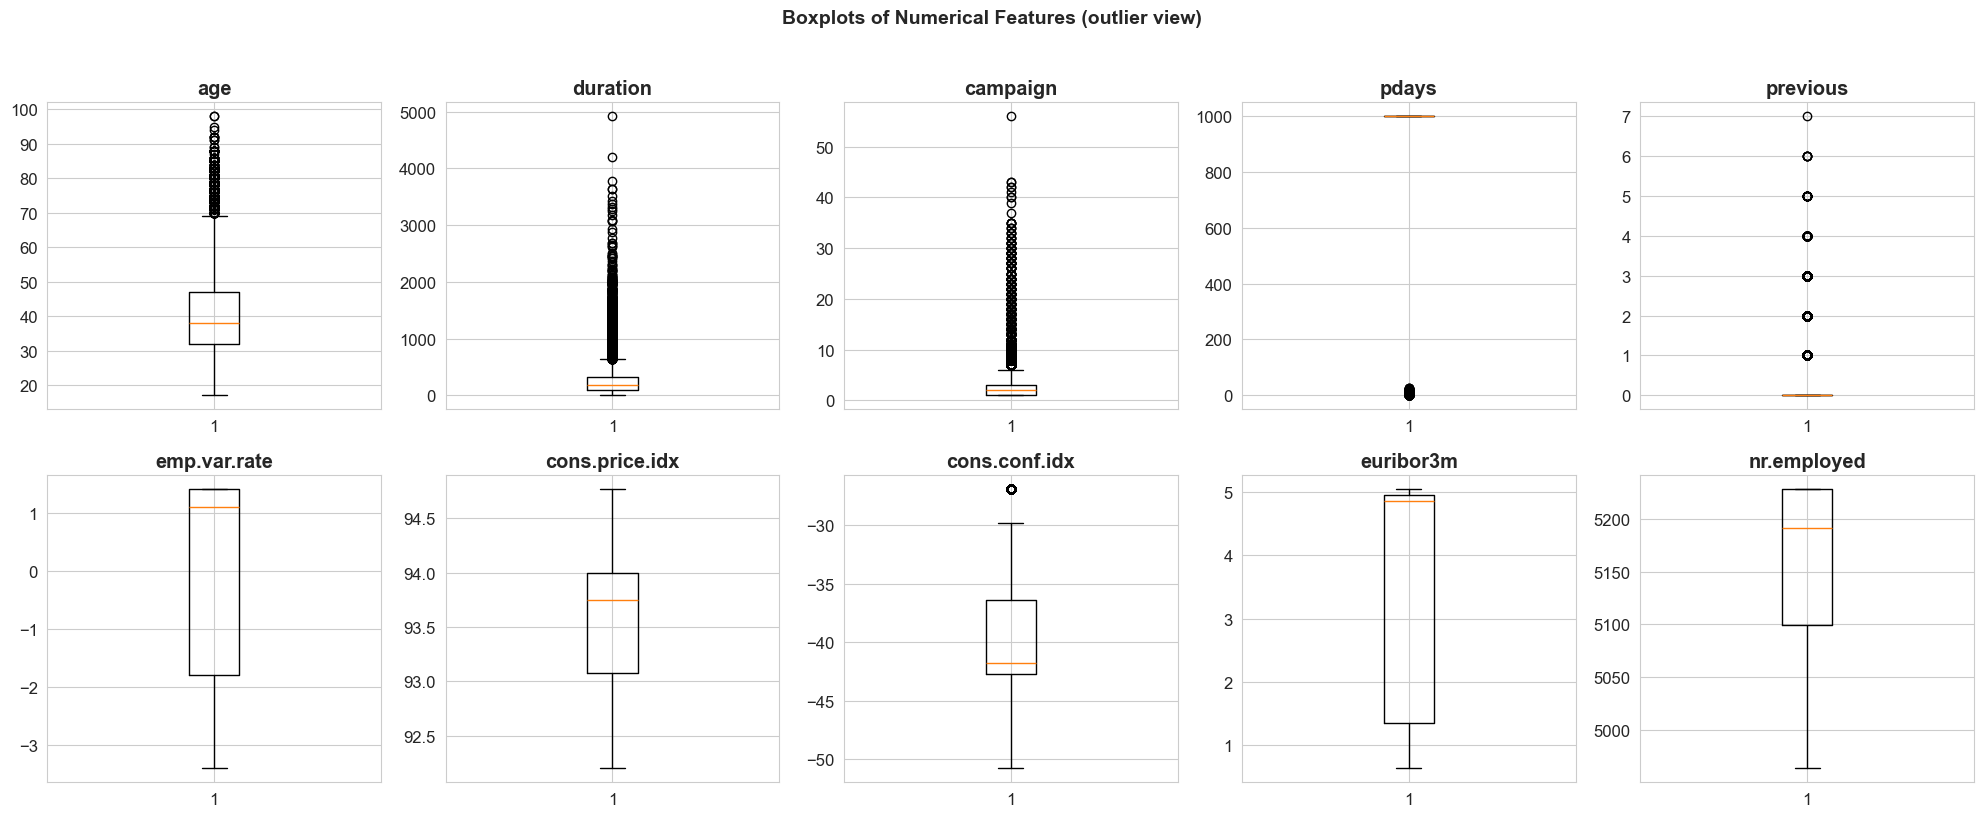
\includegraphics[width=0.92\linewidth]{preprocessing_6.png}
\caption{IQR boxplots. The flagged extremes are true values (or sentinel artifacts).}\label{fig:outliers}
\end{figure}

\section{Phase I --- Unsupervised Structural Analysis}
\paragraph{PCA.} The variance is \emph{spread} across many components: 10 out of 15 components are needed for 90\% variance and the first two PCs capture only 39\%. This is not a preprocessing failure but genuine high-dimensionality, the features span three weakly-correlated
domains, and PCA can only compress correlated ones. The loadings show those domains explicitly: PC1 (29.5\%) is the \emph{macro-economic} axis (\texttt{euribor3m}, \texttt{emp.var.rate},
\texttt{nr.employed}, all $\approx 0.45$), and PC2 (9.5\%) is \emph{campaign history} (\texttt{previous},
\texttt{poutcome}), PC3--PC5 are client-level attributes (loans, education, confidence). Dropping
\texttt{pdays} from correlated ones is justified here: if we had kept it, its sentinel would have artificially dominated PC1. For the clustering that follows we keep the first 10 components (the 90\% variance threshold), so the weaker client-level signals in PC3--PC5 are retained alongside the dominant macro and campaign axes.

\begin{figure}[H]
\centering
\begin{subfigure}{0.62\linewidth}
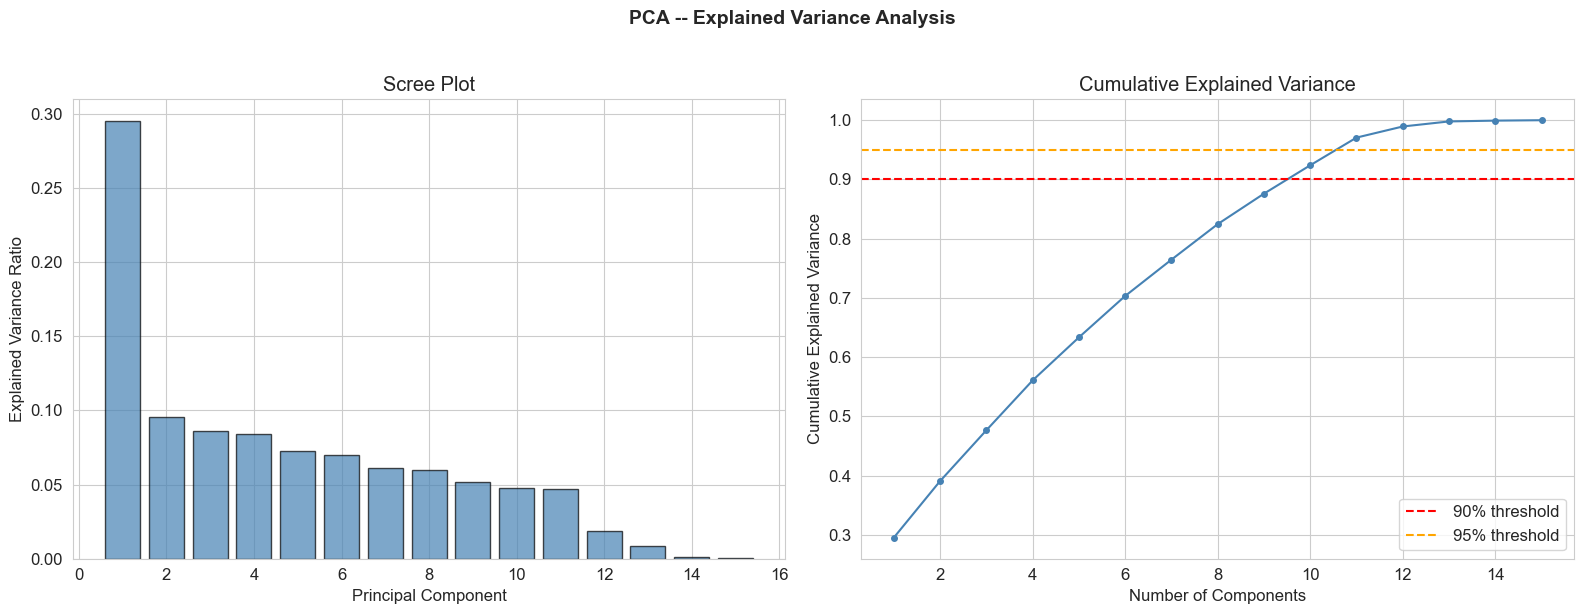
\includegraphics[width=\linewidth]{phase1_1.png}
\caption{Scree / cumulative variance: 10/15 PCs for 90\%.}\label{fig:pca-var}
\end{subfigure}\hfill
\begin{subfigure}{0.36\linewidth}
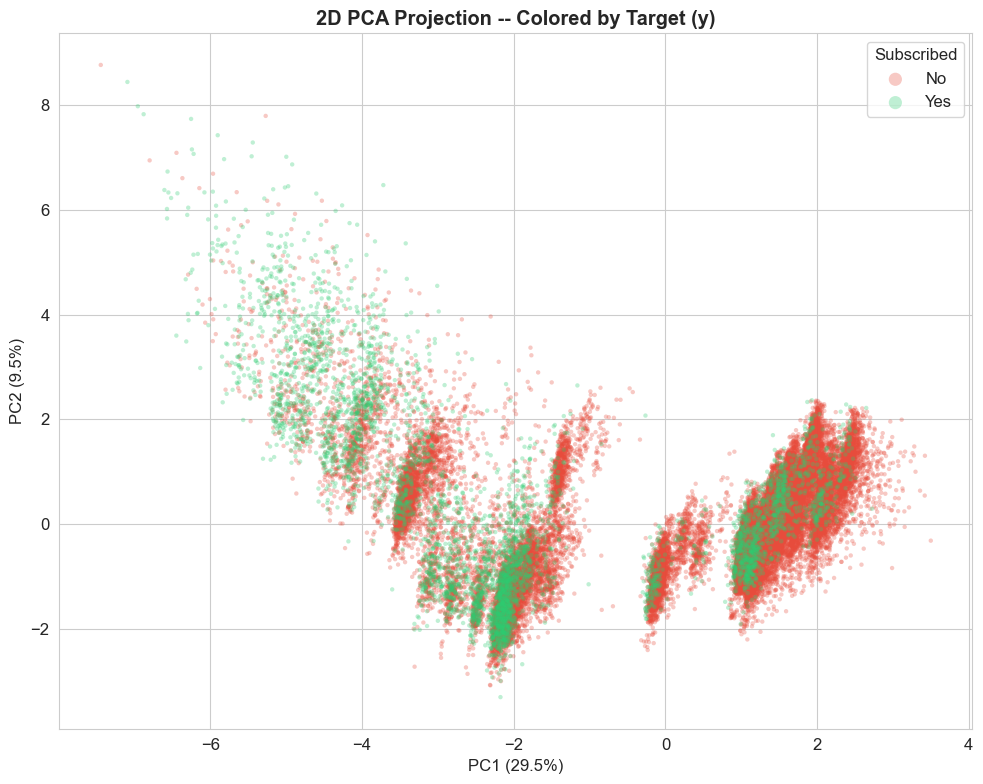
\includegraphics[width=\linewidth]{phase1_3.png}
\caption{2D PCA: heavy class overlap.}\label{fig:pca-2d}
\end{subfigure}
\caption{Phase~I --- PCA explained variance and the 2D projection coloured by target.}
\end{figure}

\newpage

\paragraph{Clusters vs.\ the target.} The 2D projection  shows heavy class
overlap with no linear separating boundary, this is an early signal that the problem is hard and
non-linear-ish. We compared K-Means and GMM on PCA-reduced vs.\ full features (PCA wins at every $k$).
Silhouette is highest at $k{=}2$ ($0.30$), but that only  splits along the macro axis. We therefore also analysed $k{=}5$, which produces a
wider, more actionable spread of segment subscription rates.
Profiling the $k{=}5$ clusters showed the warmest segment is the only one combining a favourable economy
\emph{and} prior contact, confirming the economy~$+$~campaign interaction. GMM's BIC keeps decreasing with more dimensions
(selecting $k{=}10$), has many redundant and not interesting clusters rather than a few clean clusters.



\begin{figure}[H]
\centering
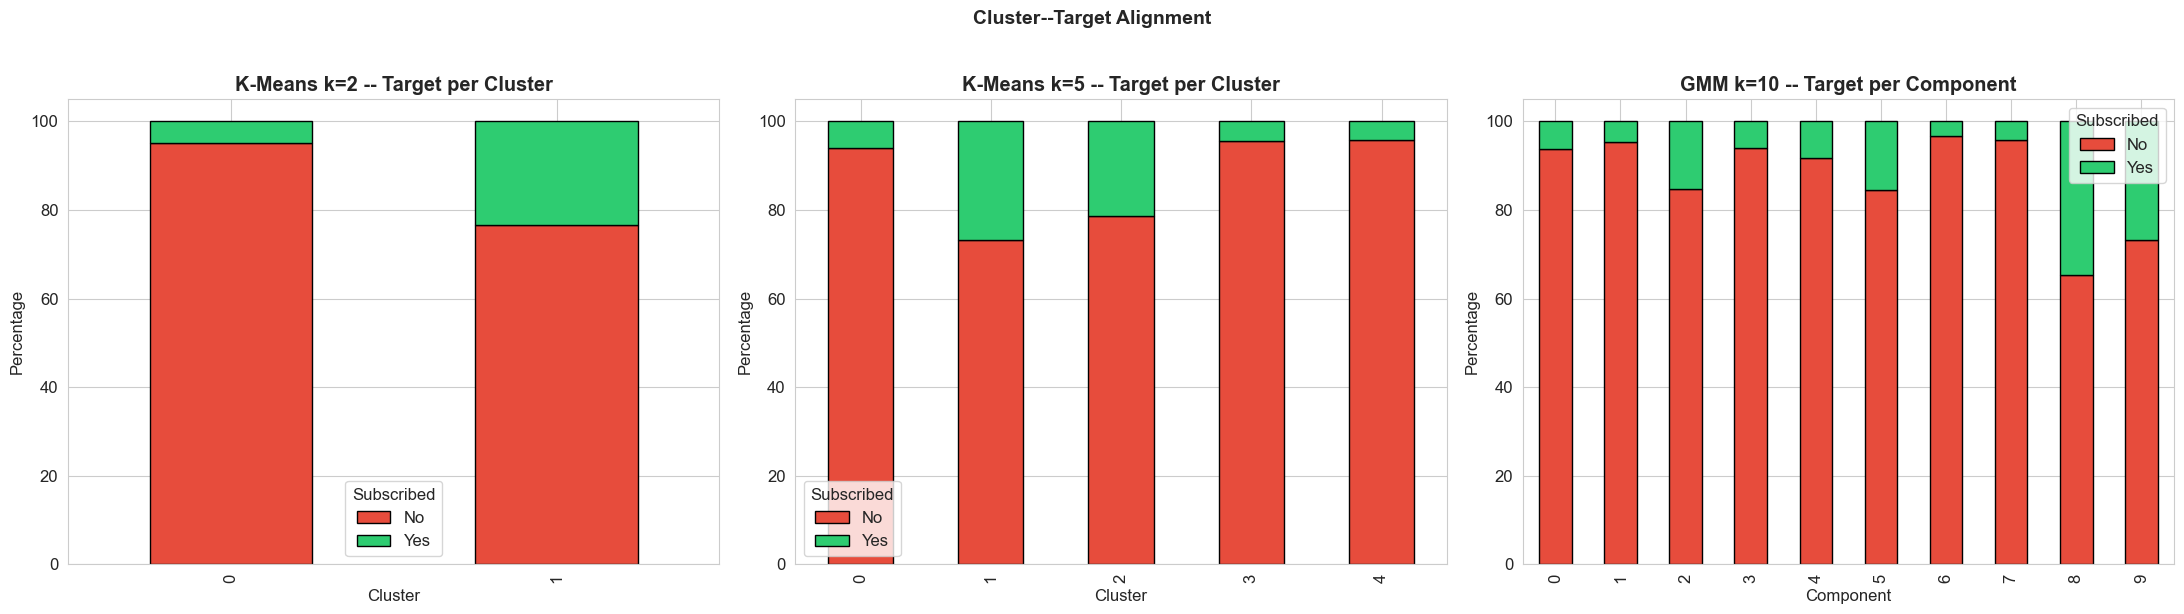
\includegraphics[width=0.95\linewidth]{phase1_7.png}
\caption{Cluster--target alignment.}
\label{fig:cluster-tgt}
\end{figure}

\section{Phase II --- Linear and Regularized Models}
\paragraph{Logistic regression.} We trained a logistic model with \texttt{class\_weight=balanced} (and
\texttt{duration} excluded) that reached test ROC-AUC~$0.797$, AUPR~$0.428$, F1~$0.46$, it recovers 64\% of
subscribers (recall) at 36\% precision, a nice recall/precision trade-off for a campaign that
wants to \emph{find} potential subscribers. The observed AUPR is approximately 4 times the 0.113 random baseline, so there is real signal despite the class overlap.

\begin{figure}[H]
\centering
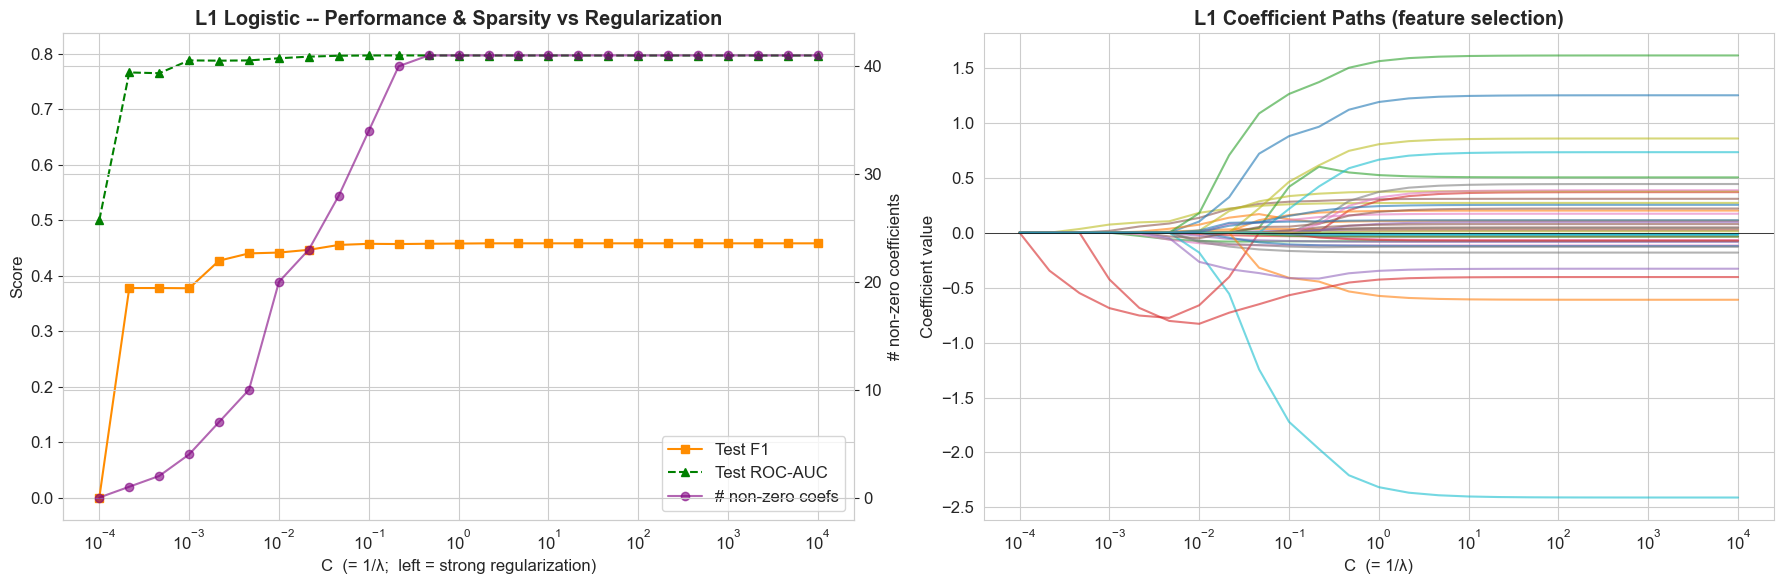
\includegraphics[width=0.95\linewidth]{phase2_3.png}
\caption{Phase~II --- L1-penalized logistic regression.}
\label{fig:l1path}
\end{figure}

\paragraph{Effect of regularization ($\lambda$).} By using the inverse strength $C=1/\lambda$
 shows that \textbf{L2/Ridge} shrinks coefficients smoothly toward zero, but never to exactly zero, whereas \textbf{L1/Lasso} drives them to \emph{exactly} zero which means performing automatic feature selection, L1 reaches almost the highest F1 (within $0.01$ of its plateau) using only
$\approx 29$ of 41 features(which is a good simplification). ROC-AUC is remarkably flat across $\lambda$ ($0.78$--$0.80$), it is mainly
the threshold-dependent F1 that suffers under heavy shrinkage. Importantly, regularization also helps tuning
the macro collinearity that we saw before, under strong $\lambda$ the three macro coefficients align and shrink together, while at weak $\lambda$ we saw that \texttt{emp.var.rate} dominates and its collinear twins flip sign (can be seen in Fig.~\ref{fig:coef}), it is directly illustrating why individual coefficients of collinear features should not be read as causal effects while regularized.

\begin{figure}[H]
\centering
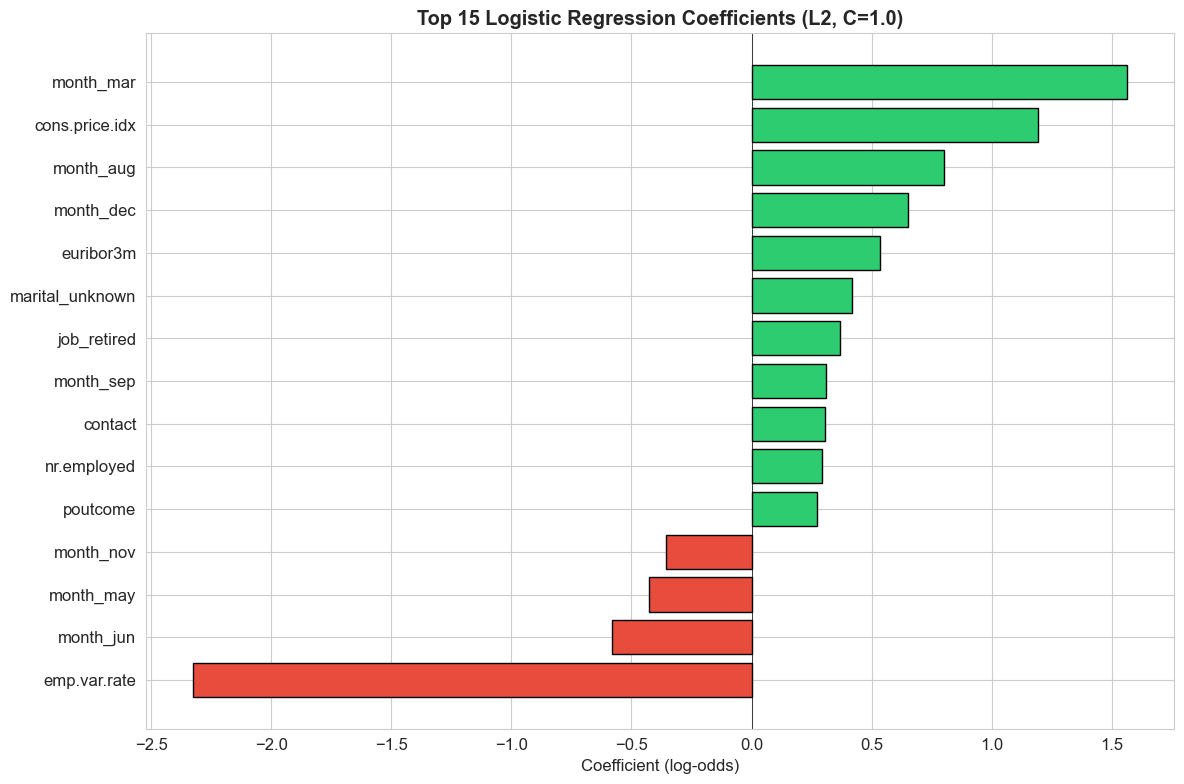
\includegraphics[width=0.7\linewidth]{phase2_7.png}
\caption{Top regularized logistic coefficients.}
\label{fig:coef}
\end{figure}

\paragraph{Ridge/Lasso as a Linear Probability Model.} Rather than inventing an artificial continuous
target, we apply Ridge/Lasso directly to the 0/1 outcome (Linear Probability Model), which allows regression and
classification to be comparable on identical features. As regression models they score only modestly
on the test set --- Ridge $R^2{=}0.21$, MAE${=}0.16$, RMSE${=}0.28$ (Lasso almost identical:
$R^2{=}0.20$, RMSE${=}0.28$). Since the target variance is just $\approx 0.10$, this barely beats
predicting the constant base rate (RMSE $\approx\sqrt{0.10}=0.32$), already a sign that squared-error
regression is a poor fit for a binary, imbalanced outcome. The deeper problem is the LPM itself: $\approx 3\%$ of its
test predictions fall \emph{outside} $[0,1]$, i.e.\ invalid probabilities, it is because The LPM models the conditional probability as a linear function of the predictors. Since linear functions are unbounded, fitted values are not restricted to the interval [0,1], and therefore some predictions may be negative or exceed one, this shows exactly why classification needs the logistic link even though the L1/L2 regularization machinery is shared.


\section{Phase III --- Kernel Methods (SVM)} We noticed that Kernel SVMs cost $O(n^2)$--$O(n^3)$, which would take a long time($\approx 15$ minutes) for full training set($\approx 33k$ samples) so we decided to grid-search linear/polynomial/RBF kernels (3-fold CV,
scored on ROC-AUC, with balanced weights) on a stratified(because of class imbalance) 12k subsample and evaluated on the full test set. All three land in a tight band: RBF and Polynomial(deg~2) are marginally best, Linear just behind, and every kernel essentially matches with Phase~II logistic model. The best hyperparameters consistently favoured smoother decision boundaries (RBF with a wide $\gamma{=}0.01$, polynomial of degree~2), telling us the data does not reward sharp non-linear boundaries, and the decision boundary is close to linear in this feature space.

\begin{table}[H]
\centering\small
\caption{Phase~III --- tuned SVM kernels (full test set).}\label{tab:svm}
\begin{tabular}{lccl}
\toprule
Kernel & ROC-AUC & AUPR & Best params \\
\midrule
RBF        & \textbf{0.793} & 0.431 & $C{=}1,\ \gamma{=}0.01$ \\
Polynomial & 0.788 & \textbf{0.436} & $C{=}1,\ \mathrm{deg}{=}2$ \\
Linear     & 0.784 & 0.384 & $C{=}0.1$ \\
Baseline   & 0.505 & 0.114 & --- \\
\bottomrule
\end{tabular}
\end{table}


\paragraph{Can engineered features break the ceiling?} Because of curiosity, we experiment adding a few interaction terms (e.g.\ economy~$\times$~effort) plus a PCA macro-composite and ran the kernels. The gain was small but revealing that \emph{linear} SVM's AUPR jumped $+0.044$ while the kernels barely moved, the explicit
interactions let the linear model express what the kernels already captured implicitly. The
$\approx 0.79$ ROC-AUC ceiling is still held, confirming the residual overlap is inherent.



\section{Phase IV --- Ensemble Methods}
Here since Tree ensembles scale comfortably, so we were able to train Random Forest (bagging), AdaBoost and Gradient Boosting on the \emph{full} 33k (with balanced weights). Ensembles are the first family to \textbf{break the linear/kernel record}: Gradient Boosting and Random Forest both reach ROC-AUC~$\approx 0.81$ and AUPR~$\approx 0.49$, clearly above logistic/SVM, and they cost around \textbf{1--5 seconds}, versus the $\sim$55\,s the linear-SVM grid alone needed on a smaller subsample. Random Forest seems to be top among all since it also shows the best F1 $0.52$ and accuracy $0.87$(but accuracy is not so reliable in our case, we focus mostly on F1), fastest at $\sim$1.2\,s, with an OOB(out-of-bag) estimate closely matches the held-out test performance.

\begin{table}[H]
\centering\small
\caption{Phase~IV --- ensembles on the held-out test set (full 33k training).}\label{tab:ens}
\begin{tabular}{lccccc}
\toprule
Model & Acc & F1 & ROC-AUC & AUPR & Fit (s) \\
\midrule
Random Forest      & \textbf{0.872} & \textbf{0.522} & 0.807 & \textbf{0.486} & \textbf{1.2} \\
Gradient Boosting  & 0.839 & 0.480 & \textbf{0.811} & 0.484 & 5.3 \\
AdaBoost           & 0.836 & 0.463 & 0.797 & 0.461 & 2.8 \\
Baseline (dummy)   & 0.804 & 0.121 & 0.505 & 0.114 & --- \\
\bottomrule
\end{tabular}
\end{table}

\paragraph{Feature importance (we included three methods).} Because the macro block is collinear, naive importance methods are unreliable, so we use three complementary views. both \emph{Permutation} and \emph{TreeSHAP} agree the leaders are the macro-economic indicators plus \texttt{contact}/\texttt{poutcome}
/\texttt{campaign}, SHAP also adds \emph{direction} (a strong economy pushes toward ``no''). We were also including the naive impurity measure, which we dropped because it over-rated \texttt{age} purely because it is continuous, permutation on other hand shows shuffling \texttt{age} barely moves ROC-AUC, matching its $r=0.03$. Thirdly, we used \textbf{grouped permutation} because it shuffles the whole correlated blocks together, which removes permutation's collinearity blind spot, and we observed that whole economy block jointly drops ROC-AUC by $\approx 0.19$ ($0.81\!\rightarrow\!0.62$), roughly $7\times$ the campaign block and $\sim$45$\times$ client demographics. Single-feature permutation was hiding this because the collinear twins compensate for each other.



\begin{figure}[H]
\centering
\begin{subfigure}{0.49\linewidth}
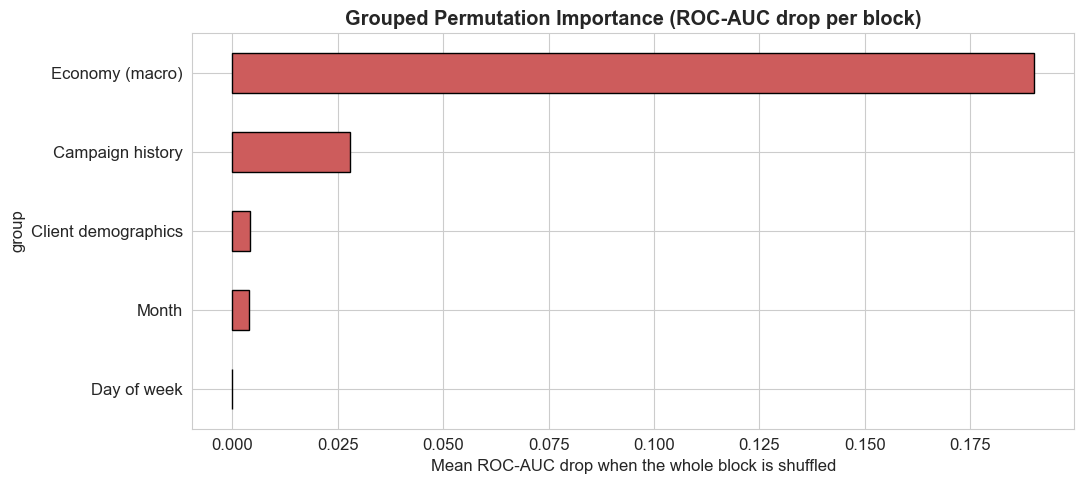
\includegraphics[width=\linewidth]{phase4_3.png}
\caption{Grouped permutation.}\label{fig:grouped}
\end{subfigure}\hfill
\begin{subfigure}{0.49\linewidth}
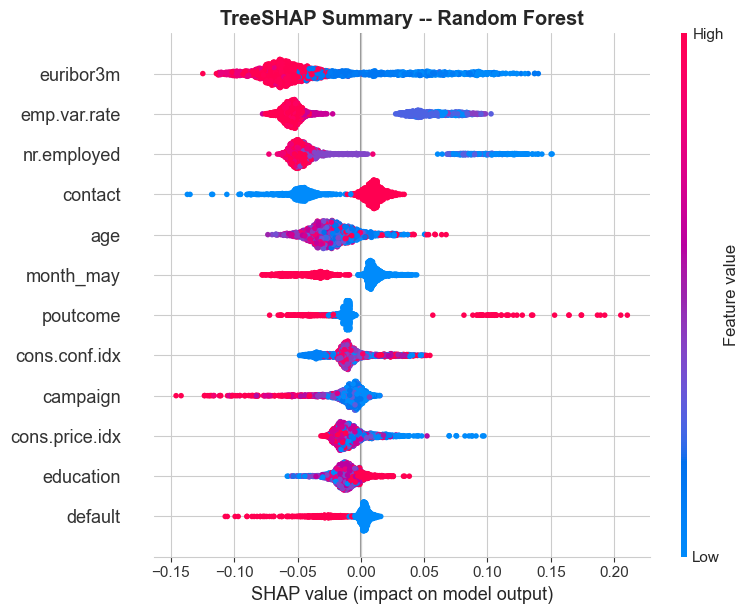
\includegraphics[width=\linewidth]{phase4_4.png}
\caption{TreeSHAP summary.}\label{fig:shap}
\end{subfigure}
\caption{Phase~IV --- feature importance. The \emph{economy block} dominates, then campaign history.}
\end{figure}

\newpage

\section{Phase V --- Model Selection and Validation}
We compared the best of each family together with the mandatory baseline using \textbf{nested cross-validation}
(inner 3-fold grid search, outer 5-fold estimate) on the full 33k, on identical folds. On full data the families separate more cleanly than using a smaller subsample to cost less time: the two
ensembles lead, above logistic and SVM, with the baseline at chance. Since the fold-to-fold spread is tiny
($\sigma\!\approx\!0.002$--$0.013$), so the ranking is stable and the boxes in the plot are also tight.

\begin{table}[H]
\centering\small
\caption{Phase~V --- nested-CV performance.}\label{tab:nested}
\begin{tabular}{lcccc}
\toprule
Model & Acc & F1 & ROC-AUC & AUPR \\
\midrule
Hist Gradient Boosting & 0.838 & 0.467 & \textbf{0.798} & \textbf{0.466} \\
Random Forest          & \textbf{0.865} & \textbf{0.494} & 0.792 & 0.466 \\
Logistic Regression    & 0.823 & 0.442 & 0.785 & 0.415 \\
SVM (RBF)              & 0.836 & 0.457 & 0.775 & 0.398 \\
Baseline (dummy)       & 0.804 & 0.122 & 0.506 & 0.114 \\
\bottomrule
\end{tabular}
\end{table}

\begin{figure}[H]
\centering
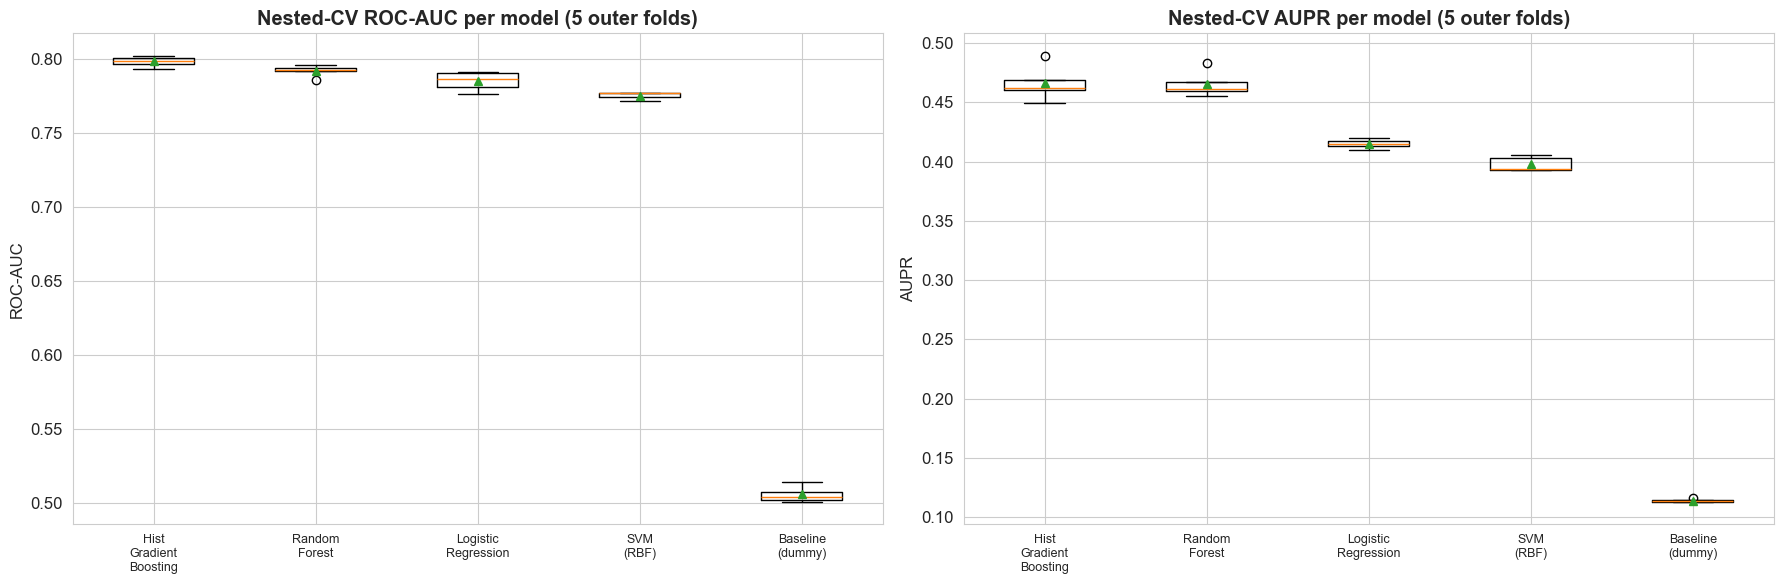
\includegraphics[width=0.95\linewidth]{phase5_1.png}
\caption{Phase~V --- nested-CV distributions over the 5 outer folds.}\label{fig:nestedbox}
\end{figure}


\paragraph{Statistical test.} We add a statistical test because the top models differ by only a few
thousandths, and picking the metric argmax would risk crowning a winner whose lead is just fold-to-fold
noise, but a paired test tells us whether a ranking difference is \emph{real} before we commit to a model. Since CV fold scores are dependent (the outer training sets overlap by $\approx 4/5$), and we used a naive paired $t$-test which was over-optimistic, we then added the \textbf{Nadeau \& Bengio
corrected resampled $t$-test} ($\rho{=}1/(k{-}1)$). It changes the conclusion exactly where it should:
the naive test called HistGB~$>$~RF on ROC-AUC ``significant'' ($p{=}0.015$), but corrected test rejects it ($p{=}0.054$), on AUPR they are a clear tie ($p{=}0.92$) by both tests. So the two ensembles are
statistically indistinguishable on both ranking metrics. With AUPR (the imbalance-appropriate metric)
tied, we break the tie by F1, because it is the only remaining metric that directly measures
minority-class quality(accuracy cannot be reliable with imbalance), where \textbf{Random Forest} wins clearly, it is also faster and we already profiled that model in previous phase, we also note Gradient Boosting as its statistical equal.

\newpage

\paragraph{Final model.} We retrained the winner model on the full 33k training samples again, the chosen Random Forest scores, on the untouched test set, \textbf{ROC-AUC:~$0.807$, AUPR:~$0.486$, F1:~$0.52$},
it recovers 62\% of subscribers at 45\% precision, which is the best precision/F1 balance observed in our project, and obviously above the baseline. The nested-CV means seen before in model selection are slightly lower than final training results, because each fold trains on only $4/5$ of the data and is averaged over five splits, the nested estimate can be seen as a conservative one, and this as the deployed model.



\begin{figure}[H]
\centering
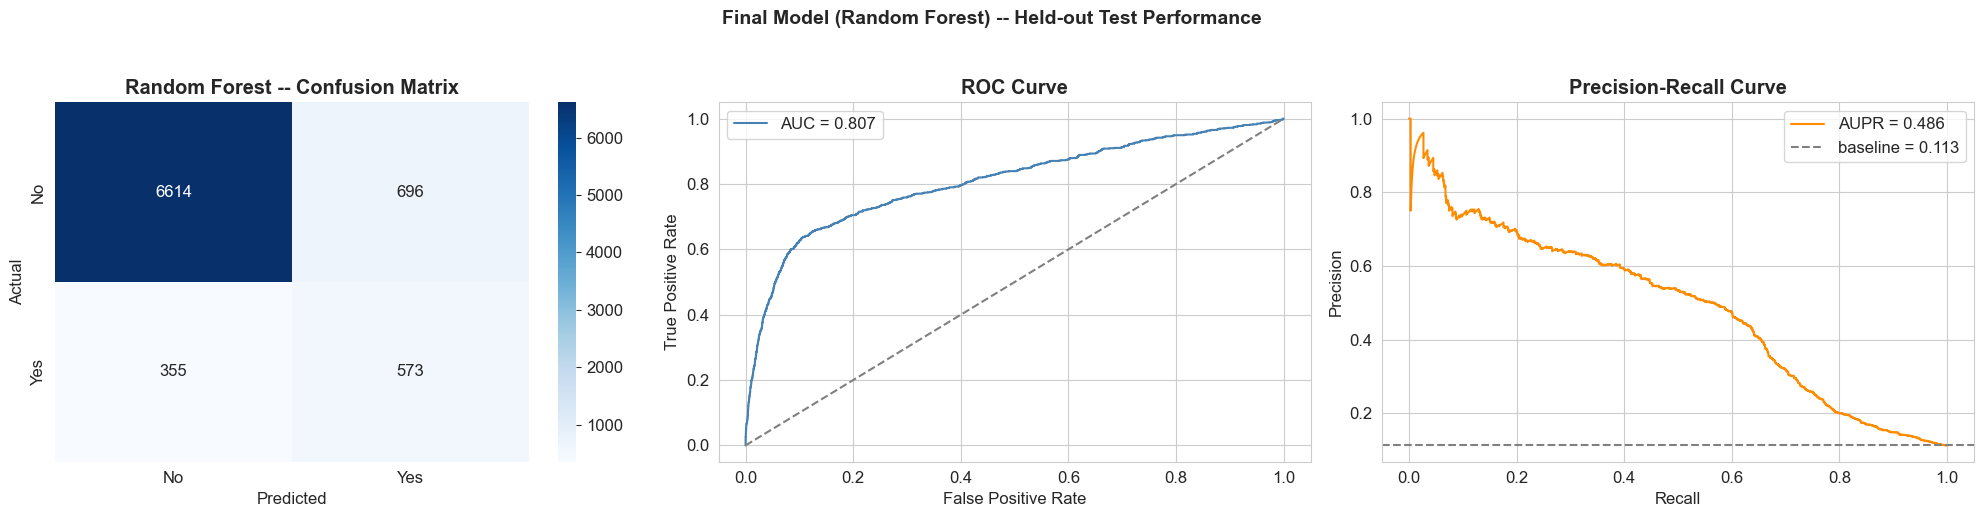
\includegraphics[width=0.95\linewidth]{phase5_2.png}
\caption{Final Random Forest on the held-out test set: confusion matrix, ROC and PR curves.}
\label{fig:final}
\end{figure}

\section{Discussion --- Dataset Challenges}
In our project we faced three challenges of this dataset. The heavy \textbf{(1) Imbalance} (11.3\%) observed between target classes pointed to never trust
accuracy as a generalization metric, and use balanced weights for all models, and evaluate focusing on AUPR/F1. The \textbf{(2) Leakage:} found in \texttt{duration} is the strongest predictor but unusable because it cant be available during real predictions, and excluding it imposes a hard ceiling,  every model family, from logistic to boosting, flattens  around ROC-AUC~$0.79$--$0.81$ / AUPR~$0.43$--$0.49$, blocked by discovered class overlap (visible in the 2D PCA). The ensembles raise this ceiling only slightly, and no method breaks it, which is consistent with the project's ``process over performance'' philosophy.
\textbf{(3) Multicollinearity:} in the macro-economic  block ($|r|>0.9$) weakens linear coefficients and fools
single-feature importance, which is why we relied on Ridge grouping, PCA and grouped permutation to read
the data honestly. The robust, cross-method conclusion  we reached is that: \textbf{economic timing} and the \textbf{prior campaign relationship} drive subscription mostly than all other features, and who the client is matters far less.

\section{Conclusions}
In this coherent five-phase pipeline of our project: PCA and clustering revealed a three-domain, class overlapping structure, while linear, kernel
and ensemble models agreed on a near-linear boundary, lastly nested CV with a corrected significance
test selected a \textbf{Random Forest} (ROC-AUC~$0.807$, AUPR~$0.486$) as the best practical model, which was 
tied with gradient boosting. For the marketing use case
the model is most valuable as a \emph{ranker}: at AUPR~$\approx 4\times$ the base rate it effectively prioritizes true subscribers at the top of the scoring list, supporting targeted marketing rather than hard classification. Future gains would require new informative features (richer client/CRM data), not a different algorithm.

\section*{Reproducibility}
All provided code is in Jupyter notebooks,
\texttt{preprocessing.ipynb} must be run first to download the data from UCI and write \texttt{data/}. Every notebook fixes \texttt{np.random.seed(42)} and \texttt{random\_state=42}, exact required package versions are pinned in \texttt{requirements.txt}. provided \texttt{README.md} file includes run order and environment setup.

\begin{thebibliography}{9}
\small
\bibitem{moro} S.~Moro, P.~Cortez, P.~Rita. \emph{A data-driven approach to predict the success of bank
telemarketing}. Decision Support Systems, 62:22--31, 2014. (UCI Bank Marketing dataset.)
\bibitem{nb} C.~Nadeau, Y.~Bengio. \emph{Inference for the generalization error}. Machine Learning,
52:239--281, 2003.
\bibitem{saito} T.~Saito, M.~Rehmsmeier. \emph{The precision-recall plot is more informative than the
ROC plot for imbalanced datasets}. PLoS ONE, 10(3):e0118432, 2015.
\bibitem{shap} S.~Lundberg, S.-I.~Lee. \emph{A unified approach to interpreting model predictions}.
NeurIPS, 2017.
\bibitem{sklearn} F.~Pedregosa et al. \emph{Scikit-learn: Machine Learning in Python}. JMLR,
12:2825--2830, 2011.
\end{thebibliography}

\end{document}
